\documentclass[a4paper,conference]{IEEEtran}

\usepackage[utf8]{inputenc}
\usepackage{graphicx}
\usepackage{hyperref}

\hypersetup{
  pdfauthor = {Guilherme Amadio and Benda Xu},
  colorlinks, urlcolor=black, citecolor=black,
  pdftitle = {Portage: Bringing Hackers' Wisdom to Science},
  pdfsubject = {Third International Workshop on HPC User Support Tools}
}

\title{Portage: Bringing Hackers' Wisdom to Science}

\author{
  \IEEEauthorblockN{Guilherme Amadio}
  \IEEEauthorblockA{São Paulo State University, Brazil\\
                    Gentoo Linux\\amadio@gentoo.org}
  \and
  \IEEEauthorblockN{Benda Xu}
  \IEEEauthorblockA{The University of Tokyo, Japan\\
                    Gentoo Linux\\heroxbd@gentoo.org}
}

\begin{document}
\maketitle

\begin{abstract}

Providing users of HPC systems a wide variety of up to date software
packages is a challenging task. Large software stacks built from source
are difficult to manage, requiring powerful package management tools.
The Portage package manager from Gentoo is a highly flexible tool that
offers a mature solution to this otherwise daunting task. The Gentoo
Prefix project develops and maintains a way of installing Gentoo systems
in non-standard locations, bringing the virtues of Gentoo to other
operating systems. Here we shall demonstrate how Gentoo Prefix
installations can be used to cross compile software packages for the
Intel® Xeon Phi™, as well as to manage large software stacks in HPC
environments.

\end{abstract}

\section{Introduction}

Building and maintaining a large software stack on an HPC environment
requires powerful packaging tools. Packages provided by the core operating
systems from HPC vendors often lag significantly behind the latest
upstream releases, while users want to make use of new features in
recent software releases, or build against specific versions of software
packages for compatibility or consistency reasons. In order to satisfy
users, the package manager must take into account the multitude of
configuration options for each package as well as ensure that the build
order is correct. It must also be able to distinguish between build
time, run time, and post build dependencies, and be able to force
package rebuilds when configuration options of dependencies change,
without rebuilding the full tree of packages in the process. Finally,
due to the particularities of each HPC environment, it is highly
desirable for the package manager to offer the ability to easily apply
patches to specific software packages. Fortunately,
Gentoo's~\cite{gentoo} Portage~\cite{gentoo:portage} package manager is
able to do all this and much more. On HPC systems where users usually do
not have permission to install software into standard locations, Gentoo
Prefix \cite{gentoo:prefix} allows installations of a Gentoo environment
into non-standard paths.

\subsection{Gentoo Linux}

Gentoo Linux \cite{gentoo} is a source-based distribution with powerful
tools that make it an excellent development environment. Gentoo has been
first released by its founder Daniel Robbins in December of 1999, and
has been in active development since then. It is a metadistribution, in
the sense that it provides the necessary tools for the user to build
his[her] own customized version of Gentoo. Gentoo uses its own package
manager, Portage~\cite{gentoo:portage}, written in Python and inspired
by the ports system from FreeBSD. Gentoo is not based on any Linux
distribution, but is itself the root of popular distributions like
Sabayon Linux, and innovative operating systems such as
CoreOS \cite{coreos} and Google's ChromeOS \cite{chromiumos}.

\subsection{Gentoo Prefix Project}
\label{sec:portage}

The Gentoo Prefix project \cite{gentoo:prefix} brings the virtues of
Gentoo Linux---such as high configurability, performance tuning, and
automated package dependency management---to different operating
systems. This is useful for installing software into systems where the
user might not have administrator privileges, or simply to use Gentoo's
Portage package manager to automate the process of fetching source code,
building, and installing software packages available in Gentoo and
having their dependencies automatically handled, including the
configuration options of each package.

Gentoo Prefix uses the host system's kernel and standard C library, but
all other tools are installed and managed during the bootstrapping of
the system. On Linux, Gentoo Prefix can also compile its own standard C
library~\cite{gentoo:rap}. Installation of the Gentoo Prefix environment
is performed by a shell script that installs the Portage package manager
into a temporary location, then uses it to bootstrap a compiler and
install the base system, which allows the user to compile and install
other sofware packages available in the Portage database. Gentoo Prefix
can be installed not only on Linux, but also on Mac OS X, BSD, AIX,
Solaris, etc. On Mac OS X, Gentoo Prefix is similar to those projects
such as Homebrew, MacPorts (source based) and Fink (binary based).

\subsection{Portage Package Manager}
\label{sec:ebuild}

Portage is a GPLv2 package management system based on FreeBSD's ports
collection. Portage consists of two main parts, the \emph{ebuild}
system, and the \emph{emerge} command line utility. The ebuild system is
responsible for executing build instructions and installing packages,
while emerge provides dependency management, and servers as the
interface to ebuild. The relationship between ebuild and emerge is not
unlike that of rpm and yum on Red Hat, and that of dpkg and apt on
Debian.

Portage packages are special bash shell scripts called \emph{ebuilds}
(not to be confused with the ebuild tool itself that is used to run
them). Ebuilds are similar to spec files in SRPMs; they contain
information on how to download, configure, compile, and install
software, as well as their dependency requirements. Gentoo's main ebuild
repository has more than 27000 ebuilds available for a variety of
architectures. Additional packages are available via official and
unofficial package overlays that complement the main tree of packages.
The special syntax used in ebuild scripts is standardized in the Package
Manager Specification (PMS) \cite{gentoo:pms} document. The PMS
documents the behavior of Portage so that Gentoo packages can be managed
by alternative package managers, such as paludis \cite{paludis} and pkgcore \cite{pkgcore}.

The Portage system has the concept of \emph{USE flags} to allow the user
to configure compile-time options of software packages. USE flags affect
which dependencies are required to build a package, which allows, for
example, a headless server to be installed with a lighter system image,
by stripping all options for building a graphical environment. USE flags
can be used in HPC systems to enable or disable MPI support, to choose
which version of the Python interpreter a module should target, to
enable specific instruction sets for a given architecture, among many
others.

For software packages that require specific versions, Portage has the
concept of package \emph{SLOTs} \cite[p.~27]{gentoo:pms}, which allow multiple versions of a same
package to be installed simultaneously on the same system. This is very
useful for, e.g., installing packages that depend on incompatible
versions of the same library, or to have multiple compiler versions
available for development and testing. SLOTs can also be used in package
dependencies to indicate when a package should be rebuilt should the
installed version of its dependencies change.

% TODO: keywords, stable/unstable/masked, patching, profiles.

\section{Gentoo Prefix on an HPC environment}
As Gentoo Prefix runs on all the GNU/Linux Distributions, it supports
GNU/Linux-based HPC systems off-the-shelf.  It is also reported that
Gentoo Prefix runs on Cray with some minor site-specific modifications
\cite{cray}.

Gentoo Prefix uses ebuilds from Gentoo main repository~(Section
\ref{sec:ebuild}) and receives cutting edge updates by 300 developers
and contributed by thousands of users.  It is a general-purpose and
full-featured environment, which mitigates a big portion of complexity
and workload of HPC software maintenance. \LaTeX{} and pandoc for
publication, emacs and vim for editing, vnc and xpra for remote
display, to name a few, are all available.

From users' point of view, Gentoo Prefix vastly expands the tools
available for HPC.  From administrators' point of view, Gentoo Prefix
supports a diversity of user needs and at the same time keep the core
operating system stable and secure. The following sections presents
several case studies to show the flexibility of Gentoo Prefix.

\subsection{Nested Job-Scheduling with Slurm}
\label{sec:slurm}
Although HPC programs are typically parallel, for some embarrassingly
parallel tasks like data analysis and simulation, it is enough to have
a grid infrastructure running many single-threaded workers divided by
input data.

Some supercomputing site allocates resources in units of nodes and
leaves finer scheduling within nodes to users.  For MPI-based parallel
programs it is straight-forward, but for single-threaded programs it
is tricky to efficiently and reliably use all the CPUs in an allocated
node.

Instead of writing \textit{ad hoc} shell scripts to launch multiple
single-threaded programs, slurm or torque available in Gentoo could be
used as a nested scheduler and allocate jobs in units of
CPUs.

\begin{figure}[htb]
  \centering
  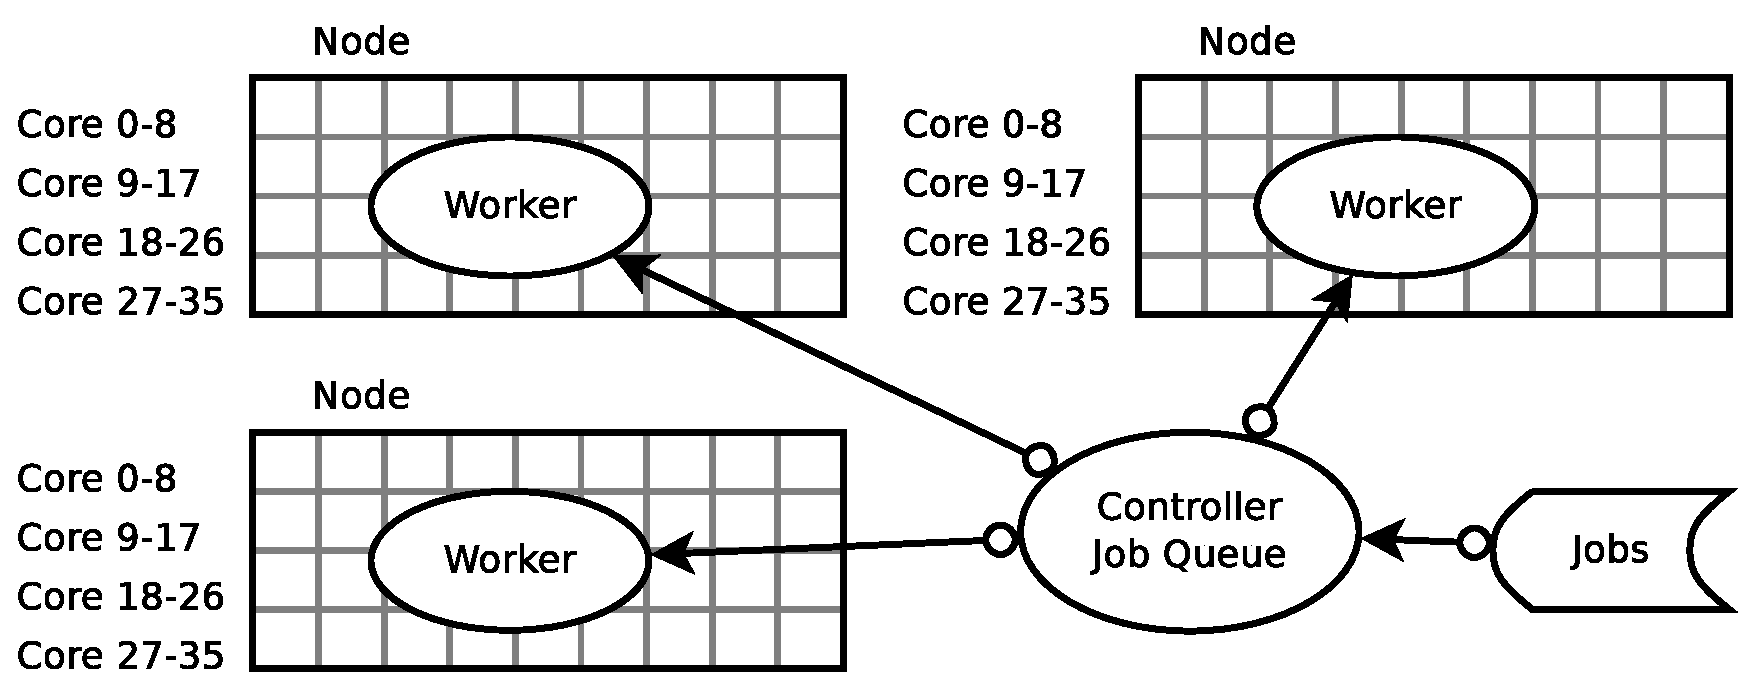
\includegraphics[width=0.5\textwidth]{node-slurm.eps}
  \caption{User slurm is nested in site PBS Pro.  The nodes are
    allocated by PBS and 1 slurm worker runs on 1 node.
    Single-threaded jobs are controlled and queued by user slurm
    controller.  Resources within a node are individually allocated.}
  \label{fig:slurm}
\end{figure}

Assume the host scheduler to be PBS Professional installed by site
administrator, the nested scheduler to be slurm installed by a normal
user with Gentoo Prefix, and the filesystem is shared between all
nodes.~(Fig.~\ref{fig:slurm}) slurm is installed by
\begin{verbatim}
$ emerge sys-cluster/slurm
\end{verbatim}
where \texttt{\$} is the normal user command line prompt.  After editing
\texttt{EPREFIX/etc/slurm/slurm.conf} to enable individual
allocation of resources within a node, slurm worker
can be launched by \texttt{slurmd} and slurm controller by
\texttt{slurmctld}.  \texttt{EPREFIX} is the installation offset of
Gentoo Prefix.

It is recommended to use munge for authentication between
\texttt{slurmd} and \texttt{slurmctld}.  OpenRC, a dependency aware
service manager, is suitable to manage the relation between munge and
slurm daemons.  Make named runlevels slurm worker and controller,
\begin{verbatim}
$ mkdir EPREFIX/etc/runlevels/worker
$ mkdir EPREFIX/etc/runlevels/controller
\end{verbatim}
Add services to the corresponding runlevels,
\begin{verbatim}
$ rc-update add munged controller worker
$ rc-update add slurmctld controller
$ rc-update add slurmd controller
\end{verbatim}
On the controller node (or login node), start slurmctld by
\begin{verbatim}
$ openrc controller
 * Starting munged ...
 * Starting slurm control daemon ...
\end{verbatim}
Submit a PBS batch script to launch slurm workers,
\begin{verbatim}
$ cat slurmd.sh
#!/bin/sh
#PBS -l select=32:ncpus=36:mpiprocs=1
#PBS -l walltime=48:00:00
source EPREFIX/etc/profile
mpirun sh -c "openrc worker; sleep 2d"
$ qsub slurmd.sh
\end{verbatim}
In the script, 32 nodes, each having 36 CPUs, are requested for 2
days. \texttt{mpirun} is used to launch 1 slurm worker per node.

After the workers are started, single-threaded jobs can be submitted
with slurm tools.

\subsection{Memory Profile with Valgrind and massif-visualizer}
\label{sec:massif}
In the context of HPC, my large scale problems could become
memory-bounded, for example when fill-in happens to a sparse matrix
based algorithm.  Valgrind is traditionally a memory debugging tool
for memory leak detection.  A heap profiler, massif~\cite{massif}, is
also distributed with valgrind.
massif-visualizer~\cite{massif:visualizer} is a handful GUI visualizer
for interpreting massif outputs besides the default CLI-based
\texttt{ms-print}.

massif-visualizer is a KDE application.  It depends on a recent KDE
framework, which is a fairly large and complex software stack.  Gentoo
Prefix readily provides the whole KDE stack thanks to the shared
\textit{ebuilds} with main Gentoo repository.  As massif-visualizer is
already in the KDE overlay, building it is straightforward,
\begin{verbatim}
$ layman --add=kde
$ emerge kde-misc/massif-visualizer
\end{verbatim}
and of course in addition to valgrind
\begin{verbatim}
$ emerge dev-util/valgrind
\end{verbatim}

To resolve the function names in the stack in valgrind output, debug
symbols are needed.  A neat feature is provided by portage to control
build environment in a per package-basis.  For example to get memory
profile of a quantile regression package \texttt{quantreg} of GNU R,
debug symbols of glibc, R and quantreg are needed. In
\texttt{EPREFIX/etc/portage/env/debug-cflags.conf},
\begin{verbatim}
CFLAGS="-O2 -ggdb -pipe"
CXXFLAGS="${CFLAGS}"
FEATURES="${FEATURES} splitdebug"
\end{verbatim}
and in \texttt{EPREFIX/etc/portage/package.env},
\begin{verbatim}
sci-CRAN/quantreg debug-cflags.conf
dev-lang/R debug-cflags.conf
sys-libs/glibc debug-cflags.conf
\end{verbatim}
and rebuild the packages,
\begin{verbatim}
$ emerge sys-libs/glibc dev-lang/R \
> sci-CRAN/quantreg
\end{verbatim}

To produce and view the memory profile,
\begin{verbatim}
R -d "valgrind --tool=massif \
> --massif-out-file=rq.prof" -f rq.R
$ massif-visualizer rq.prof
\end{verbatim}
where \texttt{rq.R} is the R script to be profiled, its content
irrelavent to the discussion here.

\subsection{Cross Compiling Software for the Xeon Phi™}

Portage can be configured to cross compile software for different
platforms. The usual way of doing so is to follow the Gentoo Embedded
Handbook \cite{gentoo:embedded} to set up the appropriate toolchain and
Portage profile. However, cross compiling for the Xeon Phi™ is somewhat
different, as only the Intel® C/C++ Compiler has full support for the
Xeon Phi™'s IMCI (Initial ManyCore Instructions) architecture, which is
quite similar to the x86 architecture, but has some subtle differences.
The fact that the Xeon Phi™ is used as a coprocessor and booting does
not follow a conventional procedure is irrelevant for cross compiling.
Once the Xeon Phi™ is properly set up, it basically works as a headless
server; users can just ssh into it and run their programs. In our setup,
a server with CentOS 7 and Intel tools installed was used to host the
Gentoo Prefix installation.

Installation instructions for Gentoo Prefix can be found on the project
website \cite{gentoo:prefix}. The \texttt{bootstrap-prefix.sh} script
automates most of the process.
\begin{verbatim}
(download script from project website)
$ chmod 755 bootstrap-prefix.sh
$ ./bootstrap-prefix.sh
(follow the instructions)
\end{verbatim}

The bootstrap process consists roughly of three stages: installing a
temporary version of portage, boostrapping a compiler using the host's
toolchain, then bootstrapping a full system with the bootstrapped
compiler. On Linux, a C library can also be part of the bootstrap
process, in which case the kernel is the only piece shared between the
host and the prefix environment.

The script works as an interactive installer; it will ask the user for
some information and discuss options based on the system being
bootstrapped on. Once the script finishes running, it will create a
\texttt{startprefix} script at the root of the bootstrapped system.
Running that script brings the user into the prefix environment, and
\texttt{emerge} and other tools become available to let the user install
more packages.
\begin{verbatim}
$ ${EPREFIX}/startprefix
Entering Gentoo Prefix /micfs/gentoo
$
\end{verbatim}
In order to install Intel C/C++ compiler it is necessary to first place
the license file in \verb|${EPREFIX}/opt/intel/licenses|, and add
\verb|Intel-SDP| to \verb|ACCEPT_LICENSE| in portage's main config file
\verb|${EPREFIX}/etc/portage/make.conf|. Then, installing is done with
\begin{verbatim}
$ emerge dev-lang/icc
\end{verbatim}

Next, it is necessary to configure the new directory where cross
compiled software will be installed. In our system, we used a separate
partition \verb|/micfs| to hold the Gentoo Prefix \verb|/micfs/gentoo|
and the cross compiled prefix \verb|/micfs/gentoo-mic|. The directory
\verb|/micfs/gentoo-mic/etc/portage| contains files to configure Portage
to use the Intel compiler, and the proper compilation flags to cross
compile for the Xeon Phi.

% include listings of PREFIX/etc/portage/{bashrc,make.conf,profile/*}
\begin{verbatim}
$ cd /micfs/gentoo-mic/etc/portage
$ cat > bashrc <<-EOF
source /path/to/icc/compilervars.sh intel64
EOF
$ cat > make.conf <<-EOF
CC=icc
CXX=icpc
MPI_C=mpiicc
MPI_CXX=mpiicpc
LD=xild
AR=xiar

CFLAGS="-mmic"
CXXFLAGS="${CFLAGS}"
EOF
\end{verbatim}

We chose Geant4 as a real world example of an application to be cross
compiled and run on the Xeon Phi. Geant4 is a toolkit for the
simulation of the passage of particles through matter. It is used at the
LHC to simulate particle collisions, and played a key role in the
discovery of the Higgs boson, announced in 2012. With everything setup,
cross compilation is done by running
\begin{verbatim}
$ emerge \
> --root=/micfs/gentoo \
> --config-root=/micfs/gentoo \
> --prefix=/ sci-physics/geant
\end{verbatim}

To confirm that the software was properly cross compiled, we can check
the architecture of the generated libraries with \verb|readelf|:
\begin{verbatim}
$ readelf -h \
> /micfs/gentoo-mic/usr/lib/libG4global.so |
> grep Machine
  Machine:              Intel K1OM
\end{verbatim}

\section{Comparison to the Alternatives}
The discussion is based on a software packaging technical report of
HEP software fundation~\cite{hsf:package}.

Gentoo runs on Linux, Mac OS X and Windows
(Section \label{sec:portage}).

Support for building and installing multiple stacks in parallel:
yes, through SLOTs.

Support for multiple variants of the same project: Multi-Rel: yes,
by Prefix-chaining.

Support setting up runtime environment for a given stack, support
multiple shell flavors: yes, by Prefix-chaining, or eselect, or
modules.

Relocation, no.

Performance, all yes.

Sys-reuse, yes, with ebuild wrappers (e.g. cctools).

Community, very active.

Unique-IDs, yes.

Integrated support for check-out of given tags or branches from the
projects repositories directly: yes.

\bibliographystyle{IEEEtran}
\bibliography{portage}
\end{document}
